\documentclass{standalone}
\usepackage{tikz}
\usetikzlibrary{arrows.meta,positioning}

\begin{document}
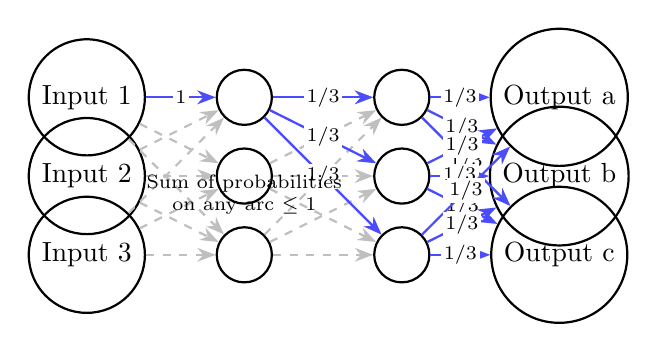
\begin{tikzpicture}[
    node distance=1.5cm,
    roundnode/.style={circle, draw=black, thick, minimum size=7mm},
    problabel/.style={font=\scriptsize, midway, fill=white, inner sep=1pt},
    blueedge/.style={-Stealth, thick, draw=blue!70},
    grayedge/.style={-Stealth, thick, draw=gray!50, dashed}
]

% Balancer structure
\node[roundnode] (In1) at (0, 2) {Input 1};
\node[roundnode] (In2) at (0, 1) {Input 2};
\node[roundnode] (In3) at (0, 0) {Input 3};

\node[roundnode] (S11) at (2, 2) {};
\node[roundnode] (S12) at (2, 1) {};
\node[roundnode] (S13) at (2, 0) {};

\node[roundnode] (S21) at (4, 2) {};
\node[roundnode] (S22) at (4, 1) {};
\node[roundnode] (S23) at (4, 0) {};

\node[roundnode] (Out1) at (6, 2) {Output a};
\node[roundnode] (Out2) at (6, 1) {Output b};
\node[roundnode] (Out3) at (6, 0) {Output c};

% Balancer connections (gray dashed for other trees)
\foreach \i in {1,2,3} {
    \foreach \j in {1,2,3} {
        \draw[grayedge] (In\i) -- (S1\j);
        \draw[grayedge] (S1\j) -- (S2\i);
        \draw[grayedge] (S2\i) -- (Out\j);
    }
}

% Blue decision tree (Input 1)
\draw[blueedge] (In1) -- node[problabel] {1} (S11);
\draw[blueedge] (S11) -- node[problabel] {1/3} (S21);
\draw[blueedge] (S11) -- node[problabel] {1/3} (S22);
\draw[blueedge] (S11) -- node[problabel] {1/3} (S23);

\draw[blueedge] (S21) -- node[problabel] {1/3} (Out1);
\draw[blueedge] (S21) -- node[problabel] {1/3} (Out2);
\draw[blueedge] (S21) -- node[problabel] {1/3} (Out3);
\draw[blueedge] (S22) -- node[problabel] {1/3} (Out1);
\draw[blueedge] (S22) -- node[problabel] {1/3} (Out2);
\draw[blueedge] (S22) -- node[problabel] {1/3} (Out3);
\draw[blueedge] (S23) -- node[problabel] {1/3} (Out1);
\draw[blueedge] (S23) -- node[problabel] {1/3} (Out2);
\draw[blueedge] (S23) -- node[problabel] {1/3} (Out3);

% Probability sum annotations
\node[below=5mm of S11, align=center, font=\scriptsize] {Sum of probabilities\\on any arc $\leq 1$};
\end{tikzpicture}
\end{document}